%%% fs-state-experiments - Experiments

\label {fs-experiments-seciton}

\subsection{Setup}
The series of experiments were performed in order to analyze the overall performance of the system's prototype. We apply building an inverted index as stream processing task for the evaluation. Building inverted index is implemented as a MapReduce transformation which is shown in Figure~\ref{index}: 

\begin{itemize}
    \item Map phase includes conversion of input documents into the key-value pairs {\it (word; word positions within the page)}
    \item Reduce phase consists of combining word positions for the corresponding word into the single index structure 
\end{itemize}

Reduce phase outputs the change records of the inverted index structure, to make this algorithm suitable for stream processing systems. It implies that each input page triggers the output of the corresponding change records of the full index. In \FlameStream\ this algorithm is implemented as the typical conversion of MapReduce transformation, which is shown in~\cite{hiddenSeim}.

\begin{figure}[htbp]
  \centering
  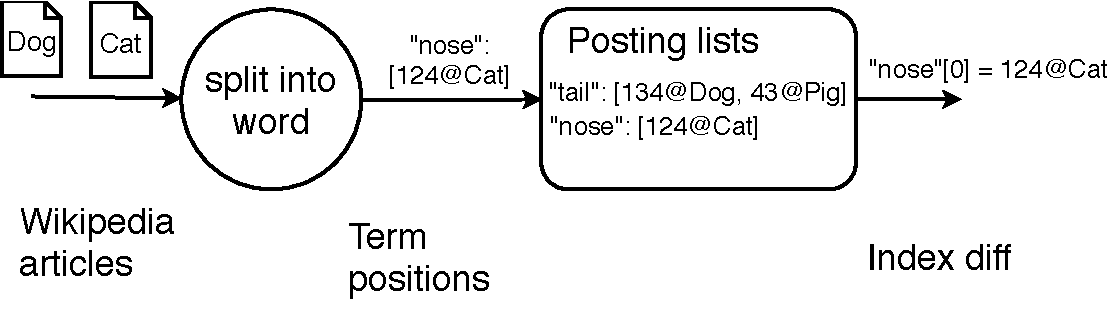
\includegraphics[width=0.50\textwidth]{pics/index}
  \caption{The inverted index pipeline}
  \label {index}
\end{figure}

We chose the task of building an inverted index because it satisfies the following properties:

\begin{itemize}
    \item The computational pipeline of the task contains network shuffle that can violate the ordering constraints. Therefore, this task is able to estimate the performance of the proposed deterministic model fairly
    \item Consistency guarantees are strongly required because the inconsistent index does not make sense for many applications
    \item The workload is unbalanced due to Zipf's law
\end{itemize}

Notably, building an inverted index in a streaming manner can be the halfway task between the generation of documents and consuming index updates by search infrastructure. In the real-world, such scenario can be found in freshness-aware systems, e.g., news processing engines.

By the notion of {\it latency} we assume the time between two events: 

\begin{enumerate}
    \item Input page is taken into the stream
    \item All the change records for the page leave the stream
\end{enumerate}

Our experiments were performed on the cluster of 10 Amazon EC2 micro instances with 1GB RAM and 1 core CPU. We used Wikipedia articles as a dataset. Documents per second input rate is 50. RocksDB~\cite{rocksdb} is used as a storage for the state. The role of data producer and data consumer is played by a custom server application that sends and receives data through socket and measures the latency.

\subsection{Overhead and recovery}
The performance of the proposed deterministic model within the same stream processing task is deeply analyzed in~\cite{hiddenSeim}. In this paper, we aim to evaluate the overhead on providing consistency guarantees and the time needed for the full recovery.

Figures~\ref{comparison50}, ~\ref{comparison500}, and ~\ref{comparison1000} shows the latencies of \FlameStream\ within distinct times between checkpoints, and at most once, at least once, and exactly once consistency semantics. As expected, the overhead on at least once and exactly once semantics is low (less than 10 ms), and it does not depend on the time between checkpoints. Slight overhead can be explained by the fact that asynchronous state snapshotting is executed on single-core nodes. The time between checkpoints does not influence latency because barrier flushing and state snapshotting mechanisms are independent in our model. The latencies under at least once and exactly once semantics are the same because the only difference between them regarding our model is in contract with data consumer.

System's behavior in case of failures and recoveries is demonstrated in Figure~\ref{recovery}. It is shown that the system can perform recovery processes in an adequate time. Existing latency spikes are caused by replay process, JVM restart, etc.

\begin{figure}[htbp]
  \centering
  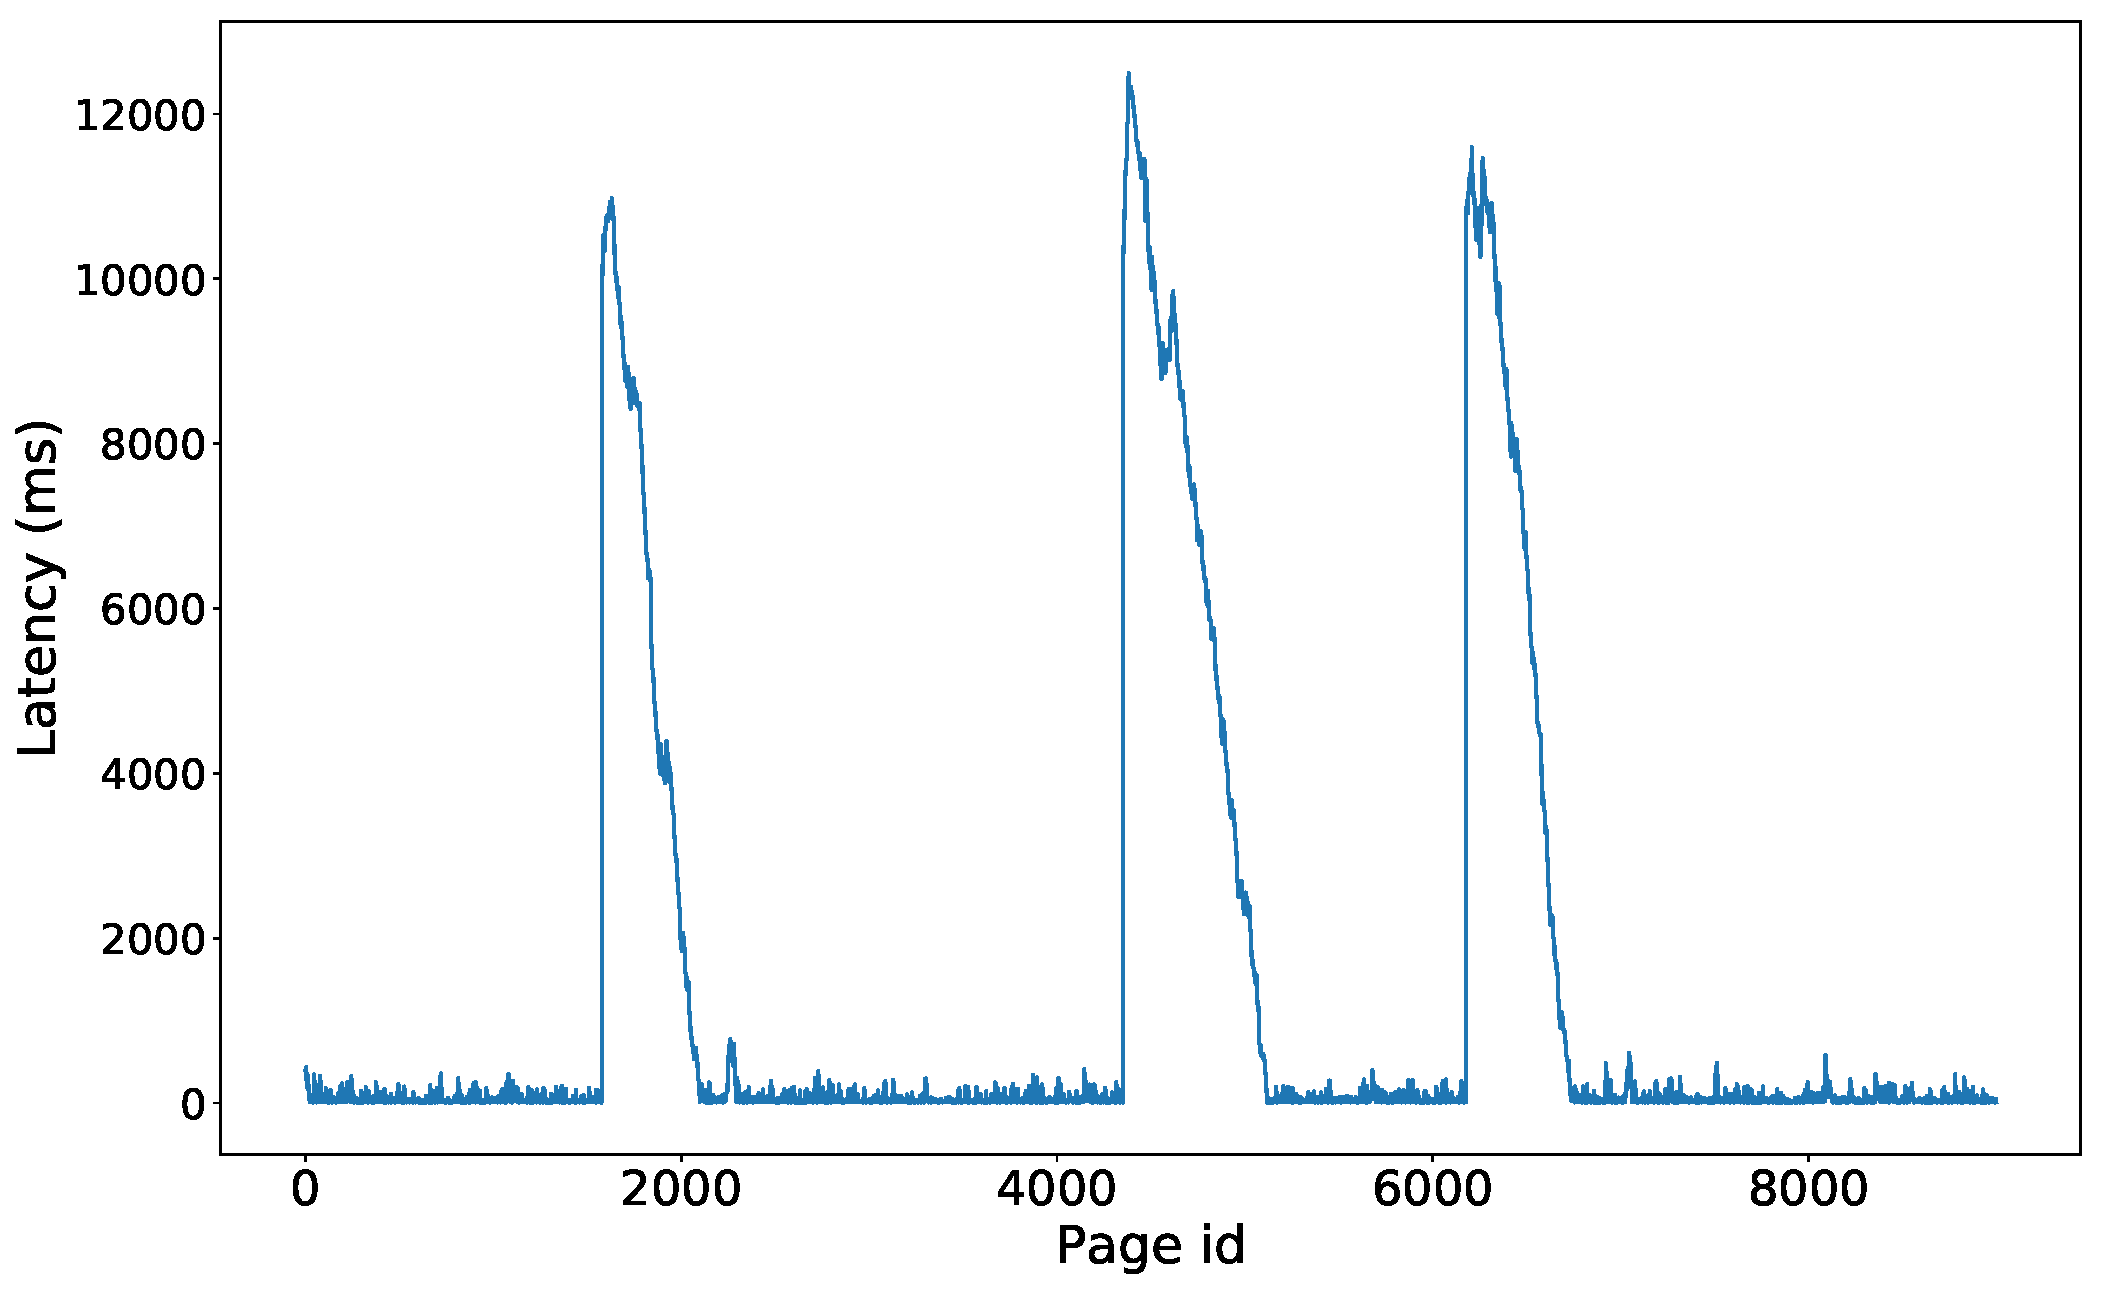
\includegraphics[width=0.48\textwidth]{pics/blink}
  \caption{The latencies of \FlameStream\ during three failures and recoveries}
  \label {recovery}
\end{figure}

\subsection{Comparison against Apache Flink}
One of the most important goals of the experiments is the performance comparison with an industrial solution regarding latency. Apache Flink has been chosen for evaluation because it is state-of-the-art stream processing system that provides similar functionality and achieves low latency in the real-world scenarios~\cite{S7530084}. 

For Apache Flink, the algorithm for building the inverted index is adopted by the usage of {\it FlatMapFunction} for map step and stateful {\it RichMapFunction} for reduce step and for producing the change records. Order enforcing before reduce is implemented using custom {\it ProcessFunction} that buffers all input until corresponding low watermark is received. Watermarks are sent after each document. The network buffer timeout is set to 0 to minimize latency. Custom {\it TwoPhaseCommitSinkFunction} that buffers output items in memory until a transaction is committed is used for experiments that require exactly-once semantics. 

{\it FsStateBackend} with the local file system is used for storing the state, because {\it RocksDBStateBackend} requires saving state to RocksDB on each update that leads to additional overhead. {\it FsStateBackend} stores state on the disk only on checkpoints and do not provide an additional overhead against RocksDB storage in \FlameStream, so it is fairer to use it rather than {\it RocksDBStateBackend} for comparison purposes.

In this paper, we compare $50^{th}$, $75^{th}$, $95^{th}$, and $99^{th}$ percentile of distributions, which clearly represent the performance from the perspective of the users' experience.

Figures~\ref{comparison50}, ~\ref{comparison500}, and ~\ref{comparison1000} demonstrates the comparison of latencies between \FlameStream\ and Flink within distinct times between checkpoints, and different consistency semantics. At the initial point, \FlameStream\ provides lower latency for at most once semantics. Such behavior is explained by the features of the optimistic approach for handling out-of-order items and is investigated in details in~\cite{hiddenSeim}. The latencies of both \FlameStream\ and Flink are slightly higher under at least once semantics. As it was mentioned above, it can be explained by the single-core configuration of the nodes. For at most once and at least once semantics, the latencies of \FlameStream\ and Flink do not vary a lot because both systems do not buffer output items for a long time before releasing. However, for exactly once semantics, Flink's latency is dramatically higher, and it directly depends on the time between checkpoints. Nevertheless, such behavior is expected, because unlike \FlameStream, Flink needs to take state snapshot and release output items within a single transaction to preserve exactly once semantics. As it was discussed above, it is the consequence of the lack of determinism in the computational model. Therefore, output items cannot be released until the transaction is committed and this fact significantly increases the latency. 

\begin{figure}[htbp]
  \centering
  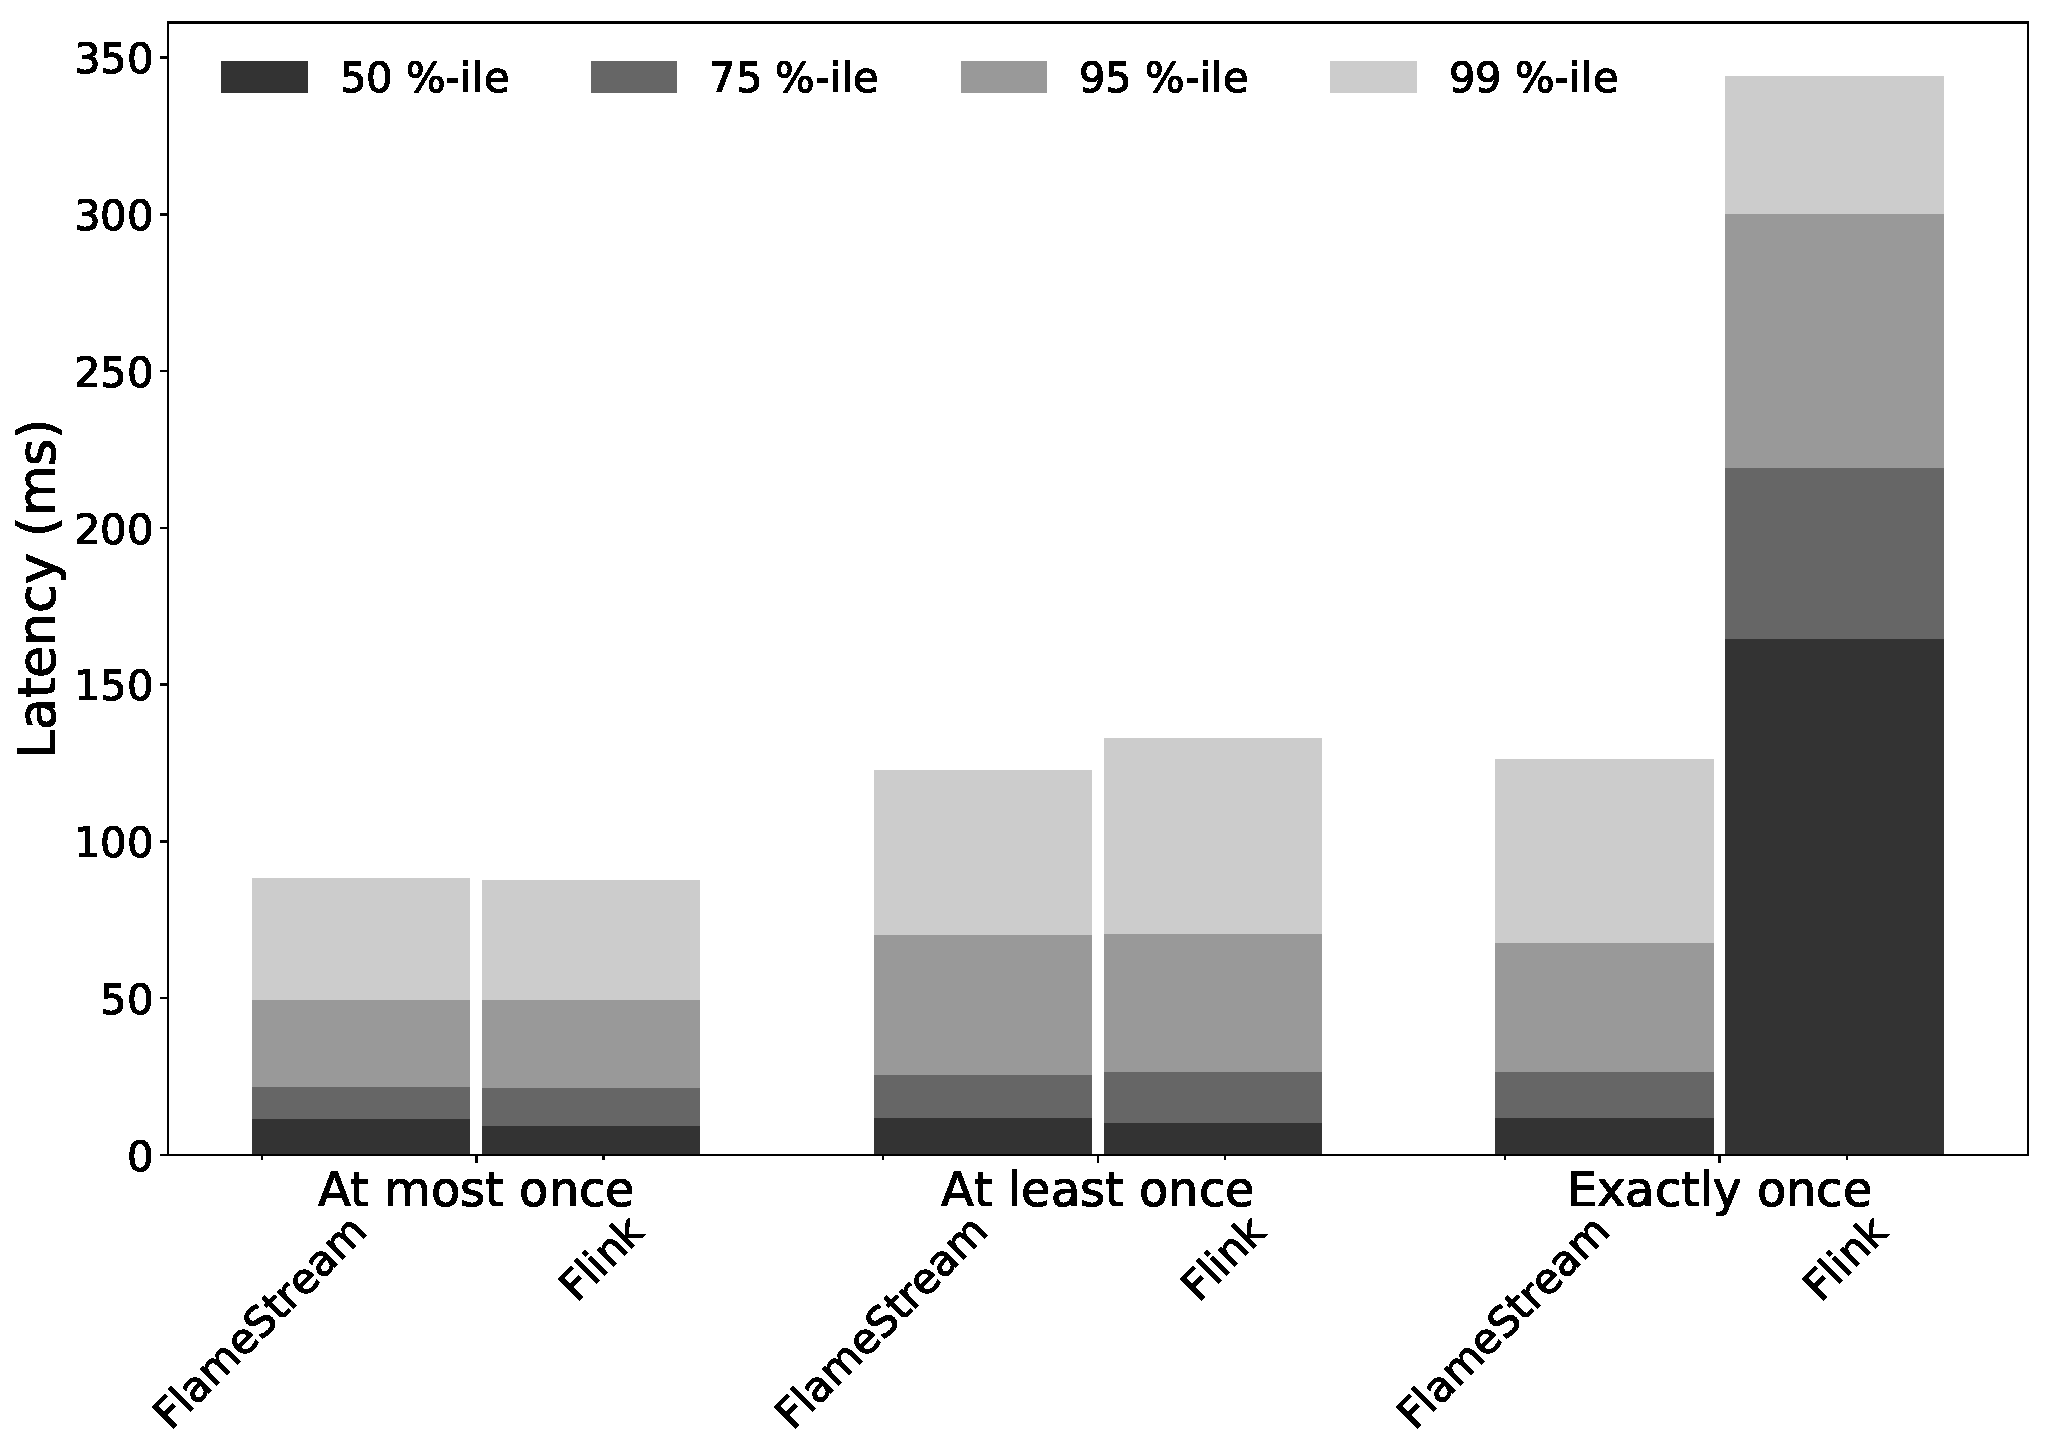
\includegraphics[width=.5\textwidth]{pics/comparison50}
  \caption{The comparison in latencies between \FlameStream\ and Flink with 50 ms delay between checkpoints}
  \label {comparison50}
\end{figure}

\begin{figure}[htbp]
  \centering
  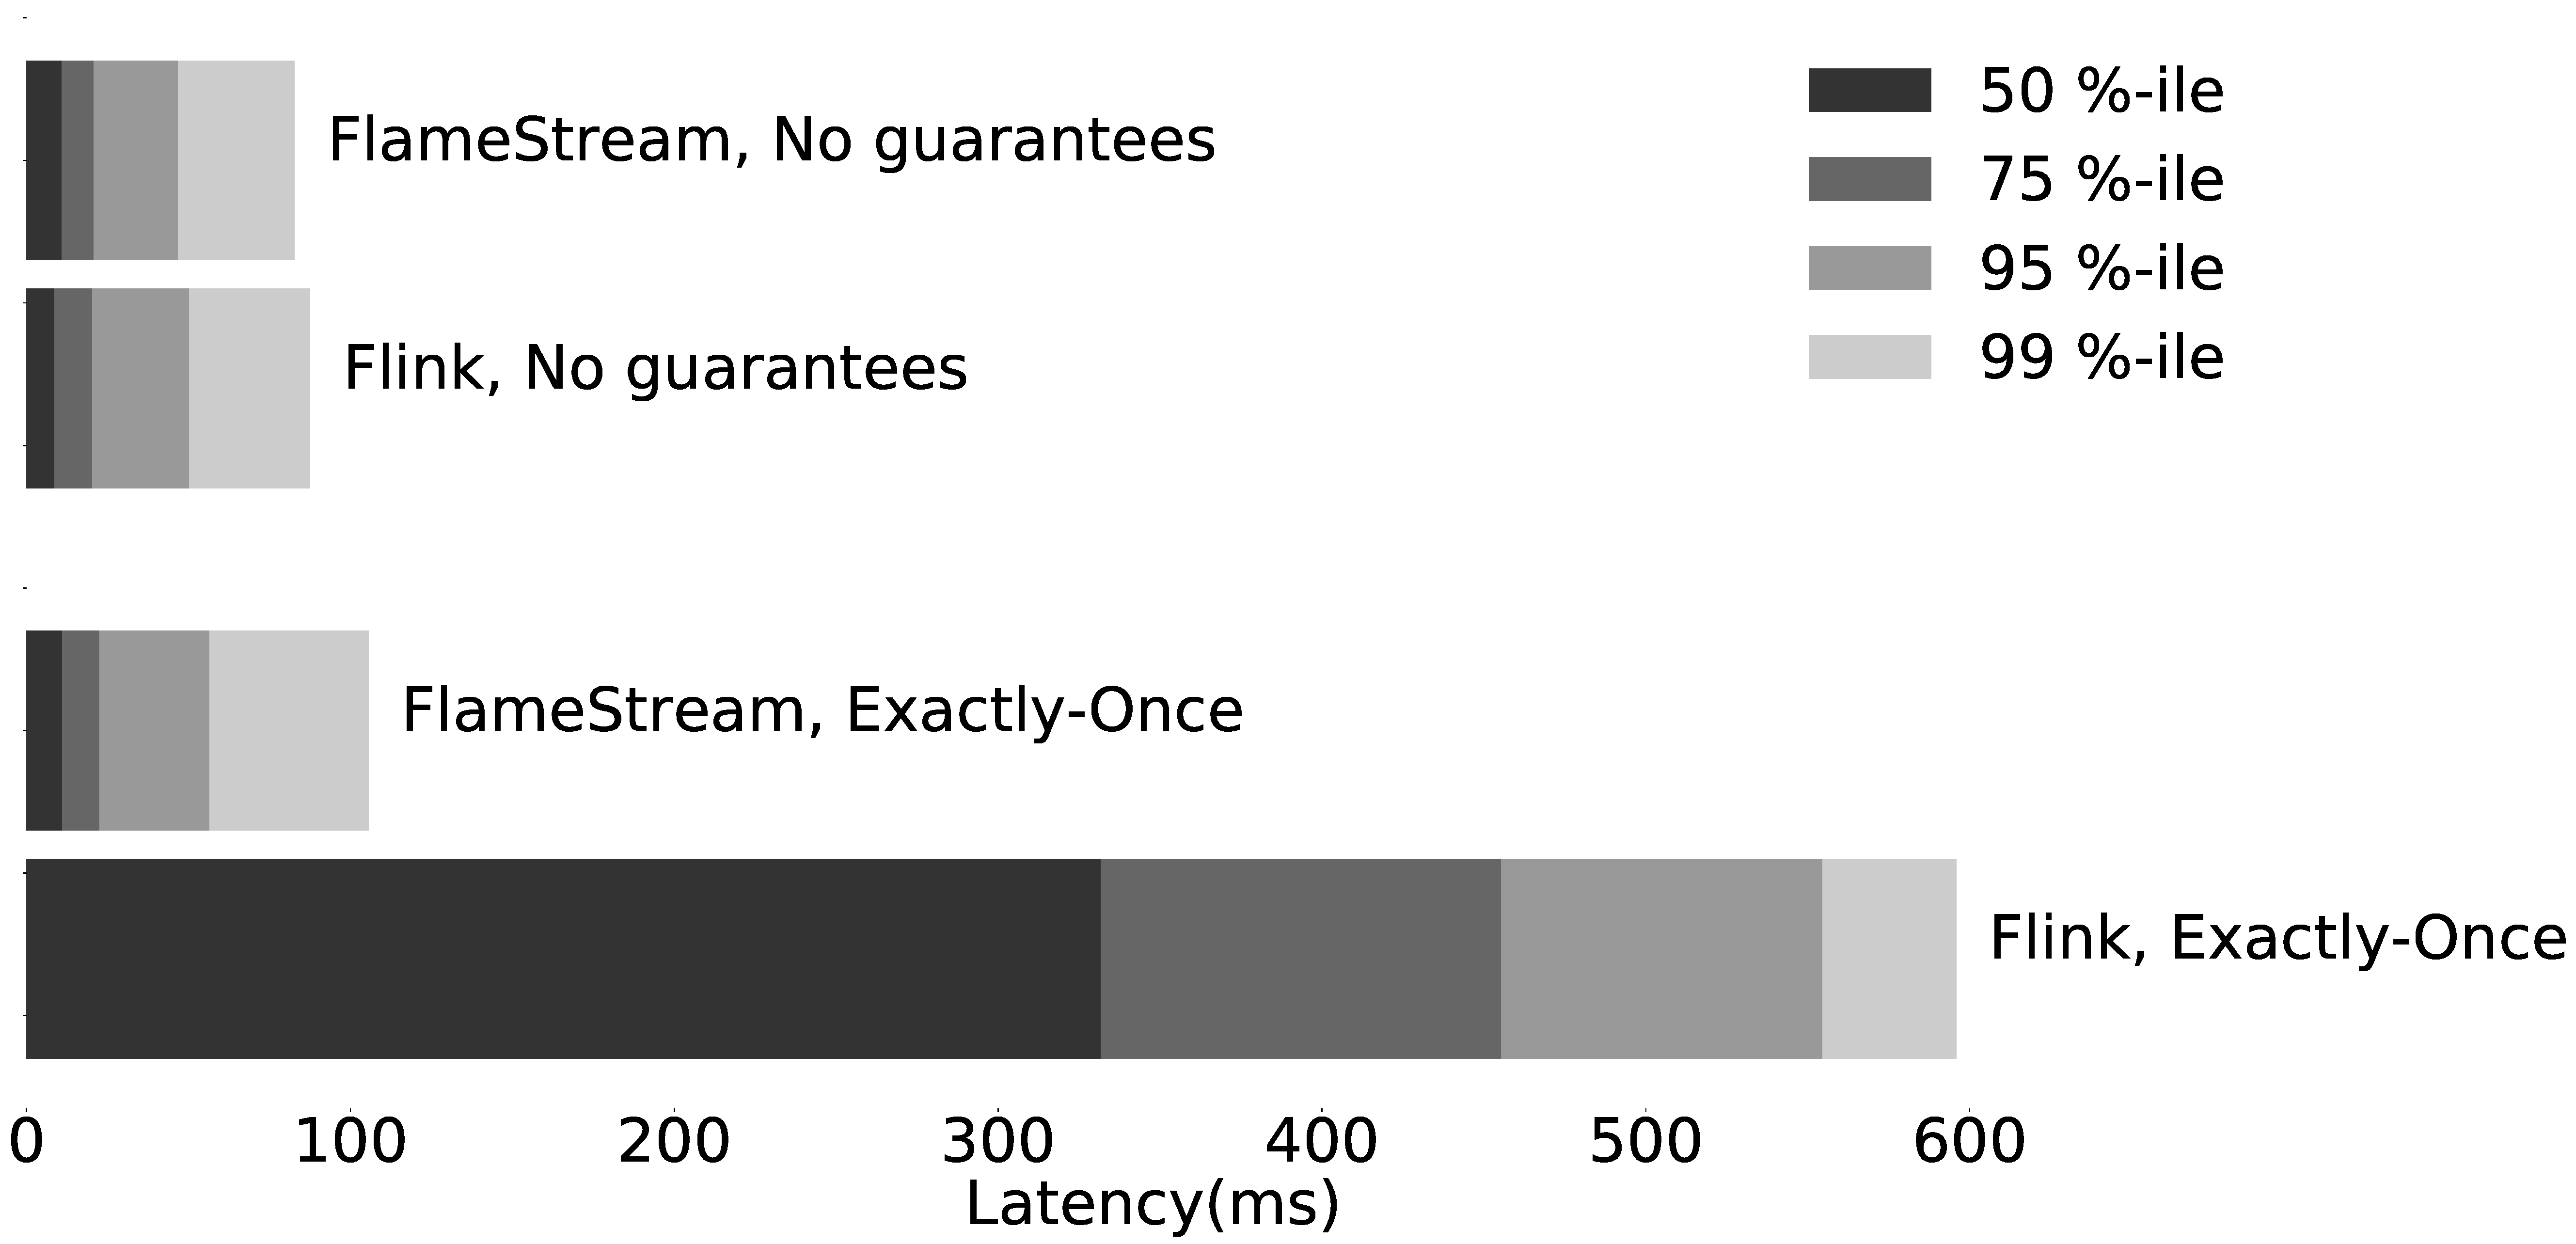
\includegraphics[width=.5\textwidth]{pics/comparison500}
  \caption{The comparison in latencies between \FlameStream\ and Flink with 500 ms delay between checkpoints}
  \label {comparison500}
\end{figure}

\begin{figure}[htbp]
  \centering
  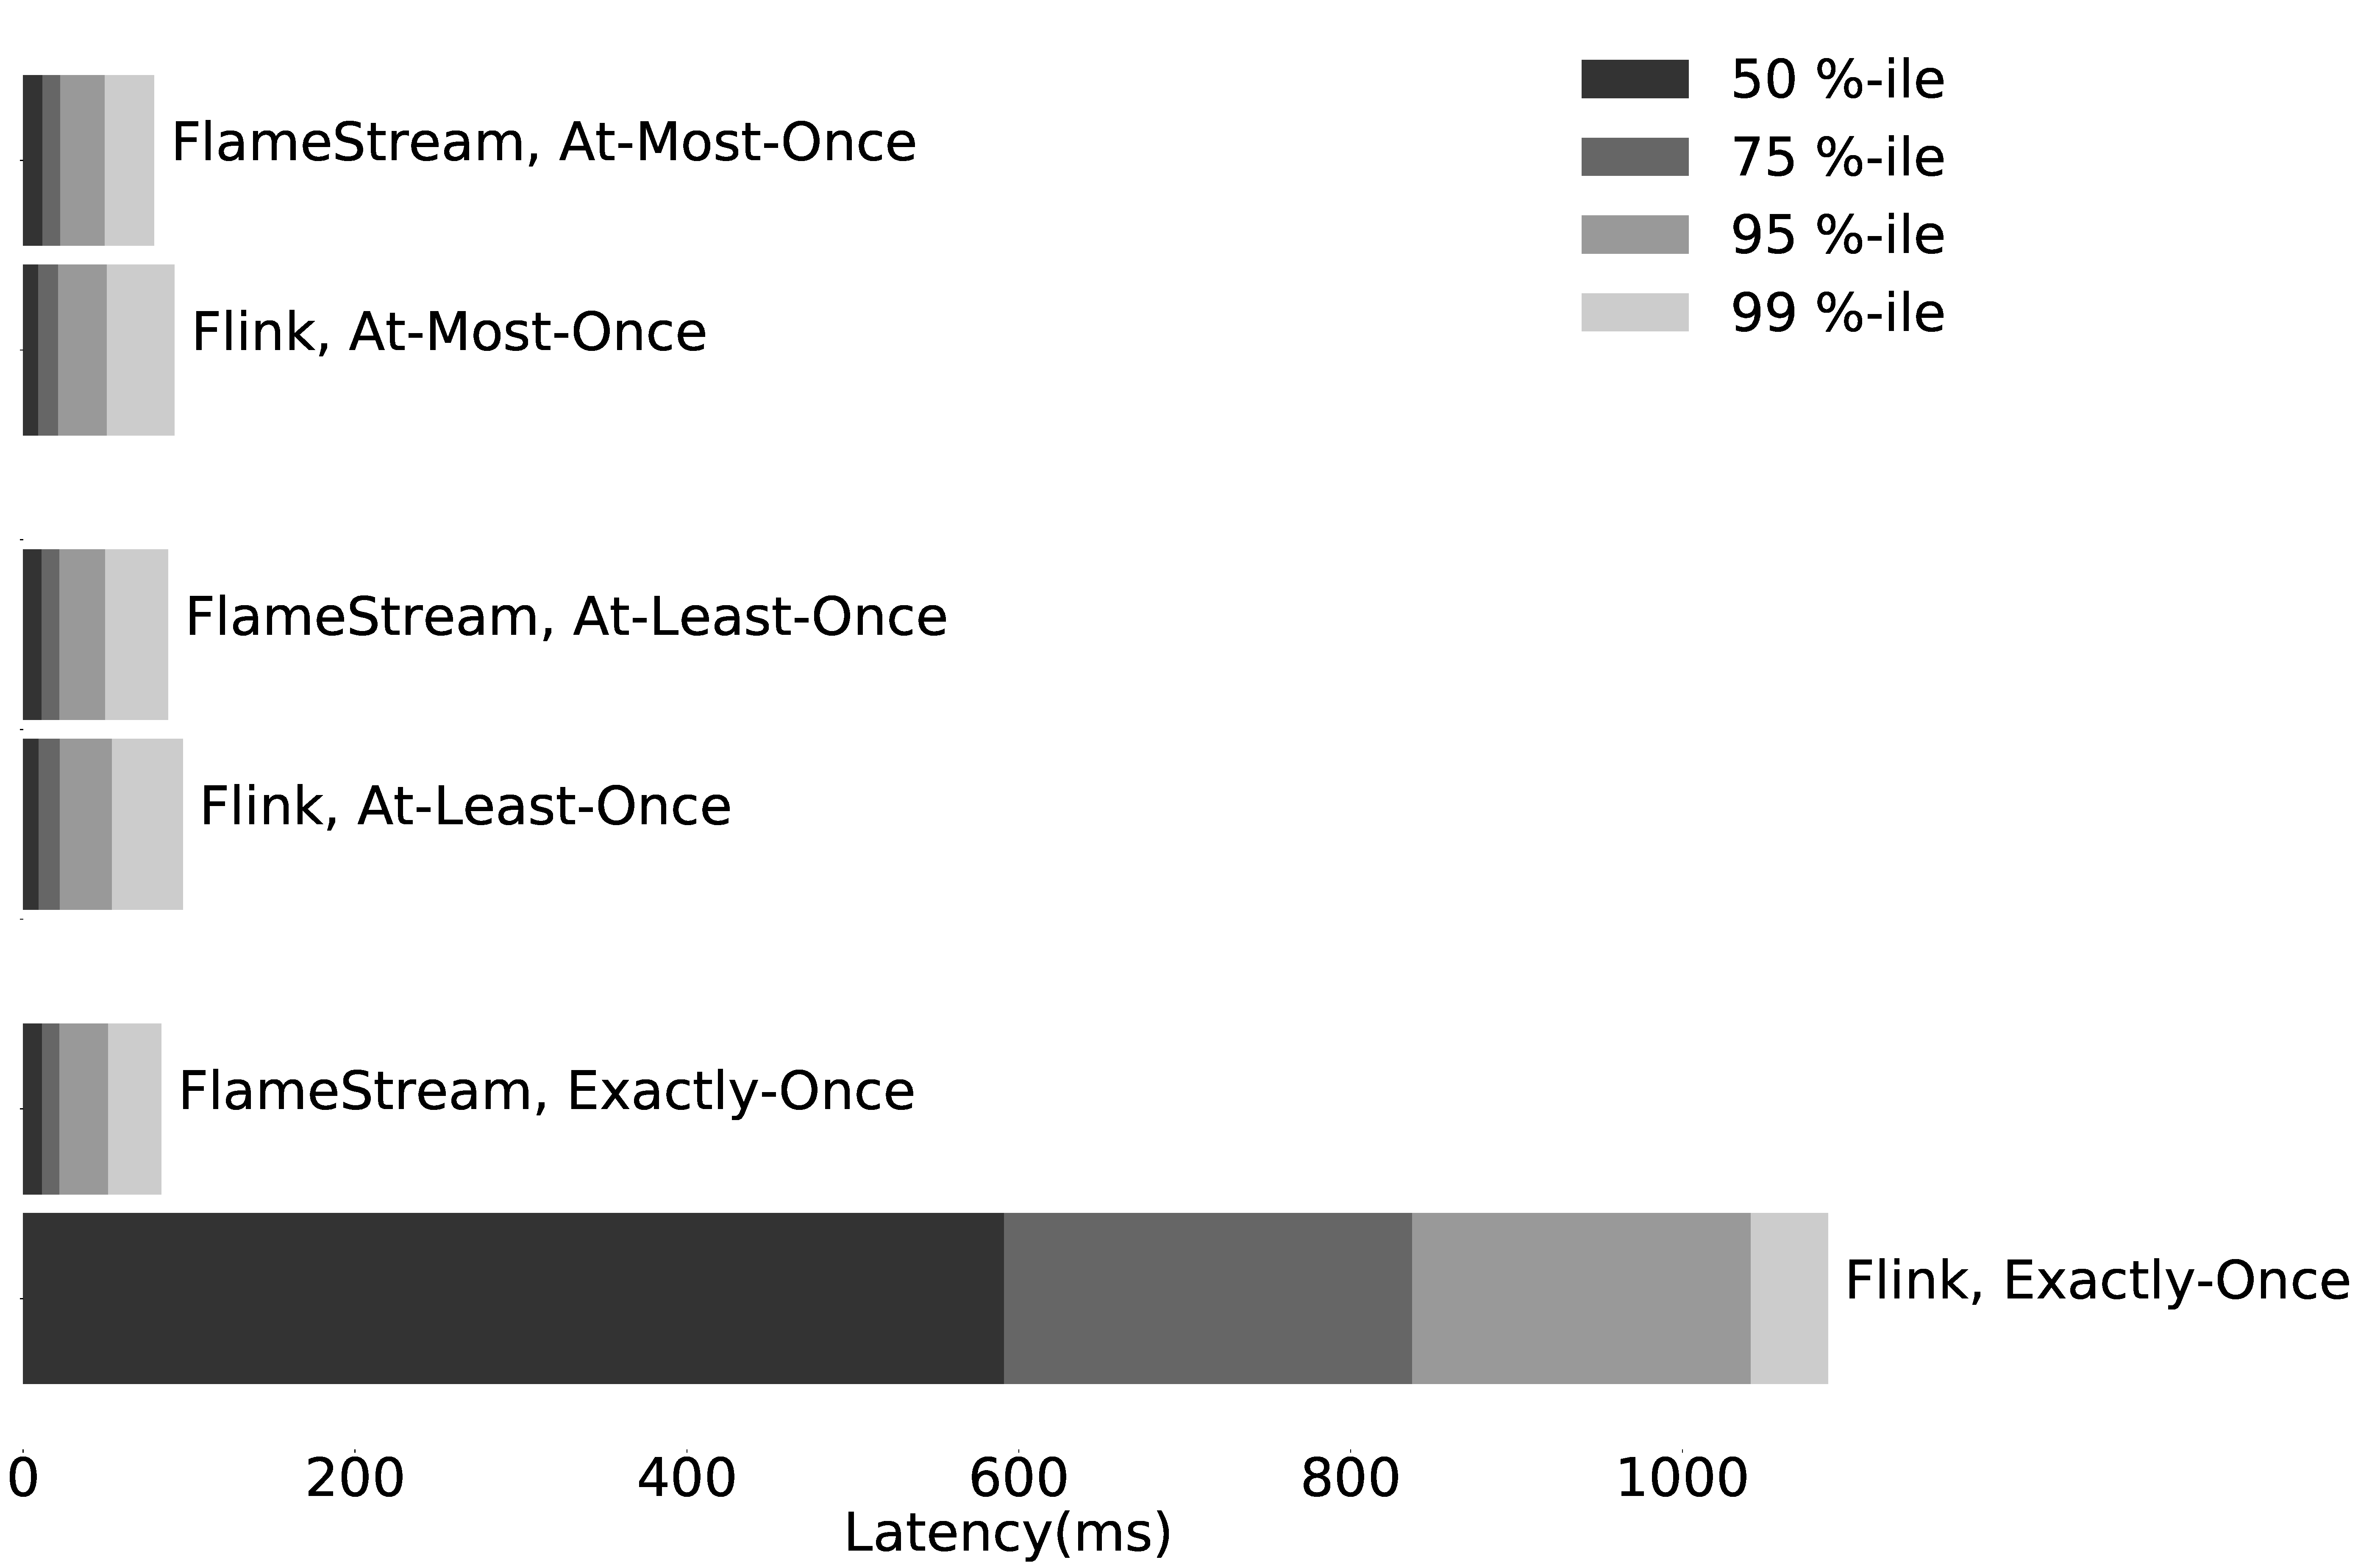
\includegraphics[width=.5\textwidth]{pics/comparison1000}
  \caption{The comparison in latencies between \FlameStream\ and Flink with 1000 ms delay between checkpoints}
  \label {comparison1000}
\end{figure}
